\documentclass{crypto-exercise}
\usepackage{pgfplots}
\usepackage{tikz}
\author{Sven Laur}
\contributor[Initial solution and proof scheme]{Kristiina Rahkema}
\editor{Sven Laur}
\tags{Discrete Logarithm problem, random self-reducibility, success amplification}
\begin{document}

\begin{exercise}{Randomised self-reducibility of the most significant bit of DL}
It is not known whether the computation of the most significant bit of discrete logarithm (MSB-DL) can be efficiently reduced to a random instance of MSB-DL. Study the consequences of such random self-reducibility by finding a lowest success probability that can be still amplified up through the majority voting.
\end{exercise}
\begin{solution} 
Let $\AD$ be an adversary that outputs the guessed significant bit $x$ for an input $y\in\GG$. Under the assumption that MSB-DL is efficiently self-reducible, we can assume that the success probability of $\AD(y)$ is $\frac{1}{2}+\varepsilon$ for each input, while the running time $t$ is still feasible. Therefore, we can run the algorithm multiple times and use majority voting to calculate the most correct answer. Let $\ADB$ be the corresponding algorithm:
\begin{align*}
    \begin{fblock}{\ADB(y)}
    &\begin{forblock}{i \in \set{1,\ldots,n}\ }
       & x_i\gets\AD(y)\\
     \end{forblock}\\
    & c \gets x_1+\cdots+x_n \\
    & \RETURN [2x > n]
    \end{fblock} 
\end{align*}
where $n$ is a fixed constant for repetitions. Although the higher number of repetition increases the success probability, it also increases the running time. Hence, we must estimate, which are the consequences of various trade-offs and which of them are in the realm of feasibility. Now let us recall the Hoeffding's inequality allows to estimate the size of the lower tail of a binomial distribution: 
\begin{align*}
\pr{x_1+\cdots+x_n\leq (p - \delta)n}\leq \exp{-2\delta^2n},
\end{align*}
where $p$ is the probability of obtaining one, i.e., $p=\pr{x_i=1}$. For the majority voting algorithm $p=\frac{1}{2}+\varepsilon$ and we must take $p-\delta=\frac{1}{2}$ to estimate failure probability. This yields
\begin{align*}
\pr{\mathsf{Failure}}=\pr{2(x_1+\cdots+x_n)\leq n}\leq \exp{-2\varepsilon^2n}\enspace.
\end{align*}
The bound shows clearly that the probability of failure $\rho$ decreases exponentially in the number of trials. However, in the context of this exercise, we are more interested how what is the lowest success probability we can amplify to the level $1-\rho$ and how it depends on the number of repetitions. Hence, we must solve the inequality $\exp{-2\varepsilon^2n} \leq\rho$ with respect to $\varepsilon$. By taking logarithm form both sides, we obtain a lower bound for $\varepsilon$: 
\begin{align*}
-2\varepsilon^2n\leq \ln\rho\quad\Leftrightarrow\quad \varepsilon\geq\sqrt{\frac{\ln(1/\rho)}{2n}}
\end{align*}  
To understand how this bound works in real life, consider a setting where the running time of $\AD$ is $1$ second on a modern computer and we are willing to use 50,000 computers throughout the year to compute the most significant bit $y$. Then the number of repetitions at our disposal is roughly $2^{40}$. The tradeoff graphs for two values of failure probability $\rho=2^{-2}$ and $\rho=2^{-80}$ are given below  

\begin{center} 
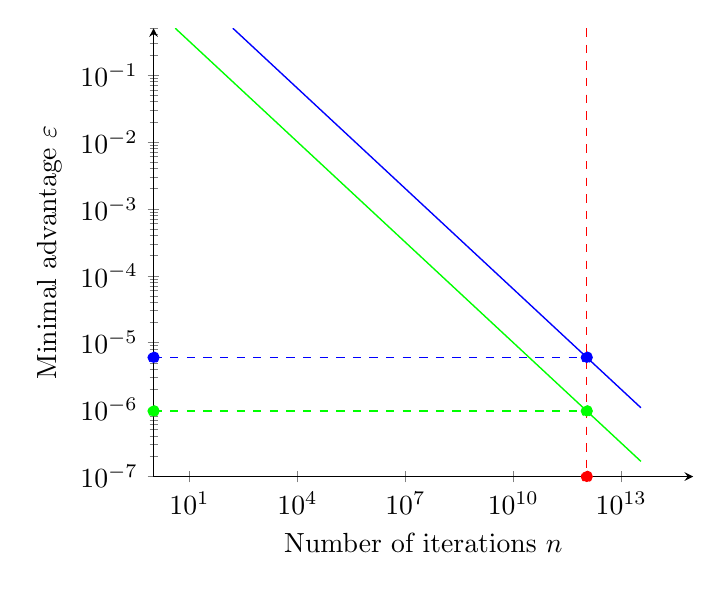
\begin{tikzpicture}
\begin{axis}[
%    y=1.5cm,              % y unit vector
%    hide y axis,          % hide the y axis
    xmode = log,          % logarithmic x axis
    ymode = log,          % logarithmic x axis
    axis x line =bottom,  % only show the bottom x axis line, without an arrow tip
    axis y line =left,
    xmin=1e0, xmax=1e15,  % range for the x axis
    ymin=1e-7, ymax = 0.5, 
    xlabel = {Number of iterations $n$},
    ylabel = {Minimal advantage $\varepsilon$},
]
\addplot [blue, line width=0.5pt] table {
160 0.5
3.518437e+13 1.06624e-06
};

\addplot [green, line width=0.5pt] table {
4 0.5
3.518437e+13 1.685874e-07
};

\addplot [red, line width=0.5pt, dashed] table {
 1.099512e+12 0.5
 1.099512e+12 1e-07
};

\addplot [green, line width=0.5pt, dashed] table {
 1e0 9.536743e-07
 1.099512e+12 9.536743e-07
};

\addplot [blue, line width=0.5pt, dashed] table {
 1e0 6.031566e-06
 1.099512e+12 6.031566e-06
};


\addplot [red, line width=0.5pt, dashed] table {
 1.099512e+12 0.5
 1.099512e+12 1e-07
};


\addplot+[only marks, mark=*, mark options={blue}] coordinates {(1e0, 6.031566e-06) (1.099512e+12, 6.031566e-06)};
\addplot+[only marks, mark=*, mark options={green}] coordinates  {(1e0, 9.536743e-07) (1.099512e+12, 9.536743e-07)};
\addplot+[only marks, mark=*, mark options={red}] coordinates {(1.099512e+12,1e-07)};


\end{axis}

\end{tikzpicture} 
\end{center}

\noindent
where the lower line corresponds to $\rho=2^{-2}$ and the higher line corresponds to $\rho=2^{-80}$. Note that even if we are willing to use significant amount of computational power, the minimal advantage is only slightly below $10^{-6}$. In another words the amplification is not very effective. Indeed, note that the lower bound of the advantage $\Theta(1/\sqrt{n})$ and thus slowdown by a factor $100$ decreases the lower bound by a factor of $10$. 

Note that for any $q$ element group $\GG$ achieving advantage of order $\frac{1}{q}$ is trivial. However, we cannot use majority voting to amplify it up to a reasonable level, since the slowdown factor would be of order $q^2$. The latter is clearly unpractical, as we can find the correct answer in $\Theta(q)$ by brute force. Thus, random self-reducibility does of MSB-DL does not imply that MSB-DL is computationally simple. Consequently, there might exists groups where MSB-DL is random self-reducible while the problem itself is hard.     

\end{solution}
\end{document}
